\documentclass{beamer}
\usetheme{tokitex}

\usepackage{graphics}
\usepackage{multirow}
\usepackage{tabto}

\usepackage[english,bahasa]{babel}
\newtranslation[to=bahasa]{Section}{Bagian}
\newtranslation[to=bahasa]{Subsection}{Subbagian}

\usepackage{listings, lstautogobble}
\usepackage{color}

\definecolor{dkgreen}{rgb}{0,0.6,0}
\definecolor{gray}{rgb}{0.5,0.5,0.5}
\definecolor{mauve}{rgb}{0.58,0,0.82}

\lstset{frame=tb,
  language=pascal,
  aboveskip=1mm,
  belowskip=1mm,
  showstringspaces=false,
  columns=fullflexible,
  keepspaces=true,
  basicstyle={\small\ttfamily},
  numbers=none,
  numberstyle=\tiny\color{gray},
  keywordstyle=\color{blue},
  commentstyle=\color{dkgreen},
  stringstyle=\color{mauve},
  breaklines=true,
  breakatwhitespace=true,
  autogobble=true
}

\title{Dynamic Programming}
\author{Tim Olimpiade Komputer Indonesia}
\date{}

\usepackage{qtree}
\begin{document}

\begin{frame}
\titlepage
\end{frame}

\begin{frame}
\frametitle{Pendahuluan}
Melalui dokumen ini, kalian akan:
\begin{itemize}
  \item Memahami konsep \foreignTerm{Dynamic Programming} (DP).
  \item Menyelesaikan beberapa contoh persoalan DP sederhana.
\end{itemize}
\end{frame}

\begin{frame}
\frametitle{Motivasi}
\begin{itemize}
  \item Diberikan $M$ jenis koin, masing-masing jenis bernilai $a_1, a_2, ..., a_M$ rupiah.
  \item Asumsikan terdapat tak hingga koin untuk setiap nominal koin yang ada. 
  \item Tentukan berapa banyaknya minimal koin untuk membayar sebesar $N$ rupiah!
\end{itemize}
\end{frame}

\begin{frame}
\frametitle{Motivasi (lanj.)}
\begin{itemize}
  \item Mari kita coba menyelesaikan masalah ini secara \fGreedy.
  \item Salah satu algoritma \fGreedy yang mungkin adalah dengan menggunakan koin terbesar yang $\leq$ sisa uang yang harus dibayar.
\end{itemize}
\end{frame}

\begin{frame}
\frametitle{Motivasi (lanj.)}
\begin{itemize}
  \item Misalkan kita memiliki nominal koin 1 rupiah, 6 rupiah, dan 10 rupiah dan ingin membayar 12 rupiah.
  \item Dengan algoritma sebelumnya, kita akan menggunakan koin 10 rupiah terlebih dahulu. 
  \item Karena tersisa 2 rupiah, berikutnya kita akan menggunakan 2 koin 1 rupiah, sehingga totalnya kita menggunakan 3 koin.
  \item Namun, ada solusi lebih baik: 2 koin 6 rupiah.
  \item Algoritma \fGreedy ini tidak memberikan solusi terbaik.
\end{itemize}
\end{frame}

\begin{frame}
\frametitle{Observasi}
\begin{itemize}
  \item Untuk membayar $N$ rupiah, kita dapat memilih salah satu koin terlebih dahulu.
  \item Jika nilai koin itu adalah $a_k$, maka sisa uang uang perlu kita bayar adalah $N-a_k$.
  \item Dalam kasus ini, terdapat $M$ pilihan koin untuk $a_k$.
\end{itemize}
\end{frame}

\begin{frame}
\frametitle{Observasi}
\begin{itemize}
  \item Perhatikan bahwa penukaran $N - a_k$ merupakan suatu sub-persoalan yang serupa dengan persoalan awalnya.
  \item Artinya, cara yang sama untuk menyelesaikan sub-persoalan dapat digunakan.
  \item Kita akan menggunakan strategi penyelesaian secara rekursif.
\end{itemize}
\end{frame}

\begin{frame}
\frametitle{Solusi rekursif}
\begin{itemize}
  \item Definisikan sebuah fungsi $f(x)$ sebagai banyaknya koin minimum yang dibutuhkan untuk membayar $x$ rupiah.
  \item Kita dapat mencoba-coba koin yang ingin kita gunakan.
  \item Jika suatu koin $a_k$ digunakan, maka kita membutuhkan $f(x-a_k)$ koin ditambah satu koin $a_k$.
  \item Atau dapat ditulis $f(x) = f(x-a_k) + 1$
  \item Pencarian nilai $f(x-a_k)$ dilakukan secara rekursif, kita kembali mencoba-coba koin yang ingin digunakan.
\end{itemize}
\end{frame}

\begin{frame}
\frametitle{Solusi rekursif}
\begin{itemize}
  \item Dari semua kemungkinan $a_k$, mana pilihan yang terbaik?
  \item Pilihan yang terbaik akan memberikan nilai $f(x - a_k) + 1$ sekecil mungkin.
  \item Jadi kita cukup mencoba semua kemungkinan $a_k$, dan ambil yang hasil $f(x - a_k) + 1$ terkecil.
\end{itemize}
\end{frame}

\begin{frame}
\frametitle{Solusi rekursif}
\begin{itemize}
  \item Jika $f(x)$ dihitung secara rekursif, apa yang menjadi \fbasecase?
  \item Kasus terkecilnya adalah $f(0)$, yang artinya kita hendak membayar 0 rupiah.
  \item Membayar 0 rupiah tidak membutuhkan satu pun koin, sehinga $f(0) = 0$.
\end{itemize}
\end{frame}

\begin{frame}
\frametitle{Solusi rekursif}
Kita implementasikan $f(x)$ sebagai fungsi $\proc{solve}(x)$:
\begin{codebox}
\Procname{$\proc{solve}(x)$}
\li \If $(x \isequal 0)$ \Then
\li   \Return $0$
\li \Else
\li   $best \gets \infty$
\li   \For $k \gets 1$ \To $M$ \Do
\li     \If $(a_k \leq x)$ \Then
\li       $best \gets \min(best, \proc{solve}(x - a_k) + 1)$
        \End
      \End
\li   \Return $best$
    \End
\end{codebox}

Jawaban akhirnya ada pada $\proc{solve}(N)$.
\end{frame}

\begin{frame}
\frametitle{Solusi rekursif}
\begin{itemize}
  \item Secara matematis, dituliskan:
   \[f(x) = \left\{\begin{array}{lr}
        0, & n = 0\\
        \min_{1 \leq k \leq M, a_k \leq x} {f(x - a_k) + 1}, & n > 0\\
        \end{array}\right. \]
 \end{itemize}
\end{frame}

\begin{frame} [fragile]
\frametitle{Solusi rekursif (lanj.)}
Mari kita lihat pohon rekursi yang dihasilkan oleh fungsi $f$. 

Berikut untuk $f(12)$ dengan nominal koin 1, 6, dan 10 rupiah.

\begin{center}
\scalebox{0.9}{
\Tree [.$f(12)$
  [.$f(2)$
    [.$f(1)$
      [.$f(0)$ ]
    ]
  ]
  [.$f(6)$
    [.$f(0)$ ]
    [.$f(5)$
      [.$f(4)$
        [.$...$
        ]
      ]
    ]
  ]
  [.$f(11)$
    [.$f(1)$
      [.$f(0)$ ]
    ]
    [.$f(5)$
      [.$f(4)$
        [.$...$          
        ]
      ]
    ]
    [.$f(10)$ 
      [.$f(0)$ 
        [.$...$ ]      
      ]
      [.$f(4)$ 
        [.$...$ ]      
      ]
      [.$f(9)$ 
        [.$...$ ]      
      ]
    ]
  ]
]
}
\end{center}
\end{frame}

\begin{frame}
\frametitle{Solusi rekursif (lanj.)}
\begin{itemize}
  \item Jika diperhatikan pada pohon rekursi, terdapat $O(M)$ cabang untuk setiap pemanggilan $f$.
  \item Untuk menghitung nilai $f(N)$, kita akan memiliki pohon rekursi yang kira-kira sedalam $O(N)$.
  \item Berarti kira-kira dilakukan $O(N^M)$ pemanggilan fungsi.
  \item Karena itu, solusi ini membutuhkan $O(N^M)$ operasi, yang mana banyaknya operasi ini eksponensial terhadap $N$ atau $M$.
\end{itemize}
\end{frame}

\begin{frame}
\frametitle{Solusi rekursif (lanj.)}
\begin{itemize}
  \item Biasanya solusi eksponensial berjalan sangat lambat.
  \item Kita tidak ingin memiliki solusi eksponensial pada pemrograman kompetitif, kecuali pada soal-soal tertentu dimana tidak terdapat solusi polinomial. 
  \item Karena itu, kita harus melakukan sebuah optimisasi.
\end{itemize}
\end{frame}

\begin{frame}
\frametitle{Optimisasi}
Jika diperhatikan, ternyata banyak $f(x)$ yang dihitung berkali-kali. Sebagai contoh, $f(5)$ dan $f(4)$.
\begin{center}
\scalebox{0.8}{
\Tree [.$f(12)$
  [.$f(2)$
    [.$f(1)$
      [.$f(0)$ ]
    ]
  ]
  [.$f(6)$
    [.$f(0)$ ]
    [.$f(5)$
      [.$f(4)$
        [.$...$
        ]
      ]
    ]
  ]
  [.$f(11)$
    [.$f(1)$
      [.$f(0)$ ]
    ]
    [.$f(5)$
      [.$f(4)$
        [.$...$          
        ]
      ]
    ]
    [.$f(10)$ 
      [.$f(0)$ 
        [.$...$ ]      
      ]
      [.$f(4)$ 
        [.$...$ ]      
      ]
      [.$f(9)$ 
        [.$...$ ]      
      ]
    ]
  ]
]
}
\end{center}
\end{frame}

\begin{frame}
\frametitle{Optimisasi}
\begin{itemize}
  \item Perhatikan bahwa hanya ada $N + 1$ kemungkinan $x$ untuk $f(x)$, yaitu $0$ sampai $N$.
  
  \item Kita dapat melakukan \newTerm{memoisasi}, yaitu mencatat hasil perhitungan $f(x)$ setelah menghitungnya.
  \item Jika suatu ketika kita kembali memerlukan nilai $f(x)$, kita tidak perlu menghitungnya kembali.
\end{itemize}
\end{frame}

\begin{frame}
\frametitle{Solusi rekursif}
\begin{codebox}
\Procname{$\proc{solve}(x)$}
\li \If $(x \isequal 0)$ \Then
\li   \Return $0$
\li \ElseIf $hasComputed[x]$ \Then
\li   \Comment Langsung kembalikan
\li   \Return $memo[x]$ 
\li \Else
\li   $best \gets \infty$
\li   \For $k \gets 1$ \To $M$ \Do
\li     \If $(a_k \leq x)$ \Then
\li       $best \gets \min(best, \proc{solve}(x - a_k) + 1)$
        \End
      \End
\li   \Comment Catat hasilnya      
\li   $hasComputed[x] \gets true$
\li   $memo[x] \gets best$
\li   \Return $best$
    \End
\end{codebox}
\end{frame}

\begin{frame}
\frametitle{Optimisasi}
\begin{itemize}
  \item Untuk menghitung suatu nilai $f(x)$, kita membutuhkan $O(M)$ iterasi.
  \item Sehingga untuk menghitung nilai $f(x)$ untuk seluruh $x$, kita membutuhkan $O(NM)$ operasi.
  \item Banyaknya operasi ini polinomial terhadap $N$ dan $M$, dan \\ \emp{jauh lebih cepat} daripada solusi rekursif sebelumnya.
\end{itemize}
\end{frame}

\begin{frame} 
\frametitle{Dynamic Programming}
\begin{itemize}
  \item Merupakan metode penyelesaian persoalan yang melibatkan pengambilan keputusan dengan memanfaatkan informasi dari penyelesaian sub-persoalan yang sama namun lebih kecil
  \item Solusi sub-persoalan tersebut hanya dihitung satu kali dan disimpan di memori.
  \item Jika sebuah persoalan adalah masalah optimisasi, maka biasanya kita mencoba semua kemungkinan solusi sub-problem yang dihasilkan, dan  mengambil yang hasilnya paling optimal. 
\end{itemize}
\end{frame}

\begin{frame} 
\frametitle{Dynamic Programming}
Terdapat dua cara mengimplementasikan DP
\begin{itemize}
  \item \newTerm{\fTopdown}: diimplementasikan secara rekursif sambil mencatat nilai yang sudah ditemukan (memoisasi).
  \item \newTerm{\fBottomup}: diimplementasikan secara iteratif dengan menghitung mulai dari kasus yang kecil ke besar.
  \newline
\end{itemize}
\end{frame}

\begin{frame} 
\frametitle{Top Down}
\begin{itemize}
  \item Cara yang sebelumnya kita gunakan adalah \ftopdown.
  \item Kata memoisasi berasal dari "memo", yang artinya catatan.
  \item Pada \ftopdown, penyelesaian masalah dimulai dari kasus yang besar.
  \item Untuk menyelesaikan kasus yang besar, dibutuhkan solusi dari kasus yang lebih kecil.
  \item Karena solusi kasus yang lebih kecil belum ada, maka kita akan mencarinya terlebih dahulu, lalu mencatat hasilnya.
  \item Hal ini dilakukan secara rekursif.
\end{itemize}
\end{frame}

\begin{frame} 
\frametitle{Bottom Up}
\begin{itemize}
  \item Pada \fbottomup, penyelesaian masalah dimulai dari kasus yang kecil.
  \item Ketika merumuskan formula rekursif, kita mengetahui jawaban kasus yang paling kecil, yaitu \fbasecase.
  \item Informasi ini digunakan untuk menyelesaikan kasus yang \\ lebih besar.
  \item Biasanya dianalogikan dengan pengisian "tabel DP".
  \item Hal ini dilakukan secara iteratif.
\end{itemize}
\end{frame}

\begin{frame}
\frametitle{Cara lain}
Secara bottom up, kita hitung semua nilai $f(x)$ untuk semua nilai $x$ dari $0$ sampai $N$ secara menaik.
\begin{codebox}
\Procname{$\proc{solve}()$}
\li $f[0] \gets 0$
\li \For $x \gets 1$ \To $N$ \Do
\li   $best \gets \infty$
\li   \For $k \gets 1$ \To $M$ \Do
\li     \If $(a_k \leq x)$ \Then
\li       $best \gets \min(best, f[x - a_k] + 1)$
        \End
      \End
\li   $f[x] \gets best$
    \End
\li \Return $f[N]$
\end{codebox}
\end{frame}

\begin{frame}
\frametitle{Top Down dan Bottom Up}
TODO: simulasi isi tabel bottom up
\end{frame}

\begin{frame}
\frametitle{Top Down dan Bottom Up}
Top Down
\begin{itemize}
  \item Sebuah transformasi natural dari formula rekursif, biasanya mudah diimplementasikan.
  \item Urutan pengisian tabel tidak penting.
  \item Hanya menghitung nilai dari fungsi jika hanya diperlukan.
  \item Ketika seluruh tabel memo pada akhirnya terisi, bisa saja lebih lambat karena adanya 
  \foverhead pemanggilan fungsi.
\end{itemize}
\end{frame}

\begin{frame}
\frametitle{Top Down dan Bottom Up}
Bottom Up
\begin{itemize}
  \item Tidak mengalami perlambatan dari \foverhead pemanggilan fungsi.
  \item Memungkinkan penggunaan teknik DP lanjutan seperti \foreignTerm{flying table}, kombinasi dengan struktur data \foreignTerm{tree}, dsb.
  \item Harus memikirkan urutan pengisian nilai tabel.
  \item Semua tabel harus diisi nilainya walaupun tidak dibutuhkan akhirnya.
\end{itemize}
\end{frame}

\begin{frame}
\frametitle{Top Down dan Bottom Up}
\begin{itemize}
  \item Beberapa orang lebih alami untuk menggunakan \ftopdown, sementara sisanya lebih terbiasa dengan \fbottomup.
  \item Bergantung dari cara berpikir Anda, salah satunya mungkin lebih mudah Anda pelajari.
  \item Untuk orang yang telah berpengalaman, penggunaan \fbottomup dan \ftopdown dapat disesuaikan dengan soal yang dihadapi.
\end{itemize}
\end{frame}

\begin{frame} 
\frametitle{Contoh Soal 1: Knapsack}
\begin{itemize}
  \item Diberikan $N$ buah barang. 
  \item Barang ke-$i$ memiliki harga $v_i$ rupiah dan berat $w_i$ gram. 
  \item Kita memiliki tas yang berkapasitas $G$ gram. 
  \item Kita ingin memasukan beberapa barang kedalam tas, sedemikian sehingga jumlah berat dari barang-barang yang kita masukan tidak lebih dari kapasitas tas dan jumlah harganya sebanyak mungkin.
\end{itemize}
\end{frame}

\begin{frame} 
\frametitle{Observasi}
\begin{itemize}
  \item Untuk setiap barang, kita harus memutuskan apakah barang ini diambil atau tidak.
  \item Jika diambil, kapasitas tas kita berkurang, dan harga barang yang kita dapatkan bertambah.
  \item Jika tidak diambil, tidak terjadi perubahan.
\end{itemize}
\end{frame}

\begin{frame} 
\frametitle{Contoh Soal 1: Knapsack (Solusi)}
\begin{itemize}
  \item Definisikan sebuah fungsi $g(x,y)$ sebagai jumlah harga maksimum yang mungkin diperoleh, jika kita hanya mempunyai barang ke-$1$ sampai ke-$x$ dan kapasitas tas kita adalah $y$ gram.
  \item Untuk menghitung fungsi $g(x,y)$ kita bisa mencoba-coba apakah kita akan memasukan barang ke-$x$ ke tas atau tidak.
\end{itemize}
\end{frame}

\begin{frame} 
\frametitle{Contoh Soal 1: Knapsack (Solusi)}
\begin{itemize}
  \item Jika kita memasukan barang ke-$x$ ke tas, maka kita akan menyisakan barang ke-$1$ sampai ke-$(x-1)$ dan sisa kapasitas tas adalah $y-w_x$. 
  \item Harga barang yang didapatkan pada kasus ini adalah $g(x-1,y-w_x)$ ditambah dengan harga yang kita peroleh pada barang ke-$x$.
  \item Dapat dituliskan $g(x, y) = g(x-1, y-w_x) + v_x$.
  \item Kasus ini hanya boleh dipertimbangkan jika $y \geq w_x$.
\end{itemize}
\end{frame}

\begin{frame} 
\frametitle{Contoh Soal 1: Knapsack (Solusi)}
\begin{itemize}
  \item Jika kita tidak memasukan barang ke-$x$ ke tas, maka kita akan menyisakan barang ke-$1$ sampai ke-$(x-1)$ dan sisa kapasitas tas masih tetap $y$.
  \item Harga barang didapatkan pada kasus ini adalah $g(x-1,y)$, tanpa tambahan apapun (kita tidak mengambil barang ke-$x$).
  \item Dapat dituliskan $g(x, y) = g(x-1, y)$.
\end{itemize}
\end{frame}

\begin{frame} 
\frametitle{Contoh Soal 1: Knapsack (Solusi)}
\begin{itemize}
  \item Dari kedua pilihan keputusan tersebut, kita tertarik dengan yang menghasilkan nilai terbesar.
  \item Cukup bandingkan mana yang lebih besar, antara:
  \begin{itemize}
    \item $g(x-1, y-w_x) + v_x$, atau
    \item $g(x-1, y)$
  \end{itemize}
  \item Dapat dituliskan: $g(x, y) = \max(g(x-1,y-w_x)+v_x,g(x-1,y))$. \newline
  \item Kembali ditekankan bahwa pilihan memasukkan barang ke-$x$ hanya boleh dipertimbangkan jika $y \geq w_x$.
\end{itemize}
\end{frame}

\begin{frame} 
\frametitle{Contoh Soal 1: Knapsack (Solusi)}
\begin{itemize}
  \item Jika $x=0$, maka berarti tidak ada lagi barang yang tersedia. 
  \item Ini berarti $g(x,y) = 0$.
  \item Kasus ini menjadi \fbasecase.
\end{itemize}
\end{frame}

\begin{frame} 
\frametitle{Contoh Soal 1: Knapsack (Solusi (lanj.))}
$g(x,y)$ dapat dirumuskan sebagai berikut:
\begin{small}
\[g(x,y) = \left\{\begin{array}{lr}
    0, & x = 0\\
    g(x-1,y), & x > 0 \wedge y < w_x\\
    \max(g(x-1,y-w_x)+v_x,g(x-1,y)), & x > 0 \wedge y \geq w_x\\
    \end{array}\right.\]
\end{small}
\end{frame}

\begin{frame} 
\frametitle{Contoh Soal 1: Knapsack (Solusi (lanj.))}
\begin{itemize}
  \item Terdapat $O(N)$ nilai berbeda untuk nilai $x$ dan $O(G)$ nilai berbeda untuk nilai $y$ pada $g(x,y)$.
  \item Dibutuhkan $O(1)$ untuk menghitung $g(x,y)$. 
  \item Sehingga untuk menghitung seluruh nilai $g(x,y)$ untuk seluruh $x$ dan $y$ dibutuhkan waktu $O(NG)$.
\end{itemize}
\end{frame}

\begin{frame}
\frametitle{Contoh Soal 1: Knapsack (Pseudocode)}
Kita implementasikan $g(x, y)$ sebagai fungsi $\proc{solve}(x,y)$:
\begin{codebox}
\Procname{$\proc{solve}(x, y)$}
\li \If $(x \isequal 0)$ \Then
\li   \Return $0$
\li \ElseIf $hasComputed[x][y]$ \Then
\li   \Return $memo[x][y]$ 
\li \Else
\li   $best \gets \proc{solve}(x-1, y)$
\li   \If $(y \geq w[x])$ \Then
\li     $best \gets \max(best, \proc{solve}(x - 1, y-w[x]) + v[x])$
      \End  
\li   $hasComputed[x][y] \gets true$
\li   $memo[x][y] \gets best$
\li   \Return $best$
    \End
\end{codebox}

Jawaban ada pada $\proc{solve}(N, G)$
\end{frame}

\begin{frame}
\frametitle{Contoh Soal 1: Knapsack (Pseudocode)}
\begin{codebox}
\Procname{$\proc{solve}()$}
\li \For $y \gets 0$ \To $G$ \Do
\li   $g[0][y] \gets 0$ \Comment Base case...
    \End
\zi
\li \Comment Isi "tabel" dari kasus yang kecil ke besar
\li \For $x \gets 1$ \To $N$ \Do
\li   \For $y \gets 0$ \To $G$ \Do
\li     $best \gets g[x-1][y]$
\li     \If $(y \geq w[x])$ \Then
\li       $best \gets \max(best, g[x - 1][y-w[x]] + v[x])$
        \End  
\li     $g[x][y] \gets best$
      \End
    \End    
\li \Return $g[N][G]$
    \End
\end{codebox}
\end{frame}

\begin{frame}
\frametitle{Contoh Soal 2: Memotong Kayu}
\begin{itemize}
  \item Kita akan memotong sebuah batang kayu dengan panjang $M$ meter pada $N$ titik menjadi $N+1$ bagian.
  \item Titik ke-$i$ berada di $L_i$ meter dari ujung kiri.
  \item Untuk memotong sebatang kayu menjadi dua, kita memerlukan usaha \alert{sebesar panjang kayu yang sedang kita potong}.
  \item Cari urutan pemotongan sedemikian sehingga total usaha yang dibutuhkan minimum!
\end{itemize}
\end{frame}

\begin{frame}
\frametitle{Contoh Soal 2: Memotong Kayu}
Sebagai contoh, terdapat sebuah kayu dengan panjang 10 meter dan terdapat 3 titik potongan pada 2 meter, 4 meter, dan 7 meter dari ujung kiri.
\begin{figure}
  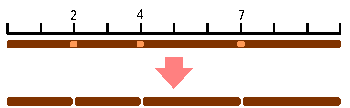
\includegraphics[width=10cm]{asset/cutting-stick-1.pdf}
\end{figure}
\end{frame}

\begin{frame}
\frametitle{Contoh Soal 2: Memotong Kayu}
Kita bisa memotong pada titik 2, titik 4, lalu titik 7 dan memerlukan usaha 10 + 8 + 6 = 24.
\begin{figure}
  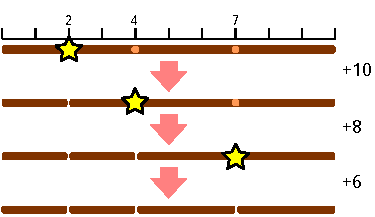
\includegraphics[width=10cm]{asset/cutting-stick-2.pdf}
\end{figure}
\end{frame}

\begin{frame}
\frametitle{Contoh Soal 2: Memotong Kayu}
Cara lain adalah memotong pada titik 4, titik 2, lalu titik 7 dan memerlukan usaha 10 + 4 + 6 = 20.
\begin{figure}
  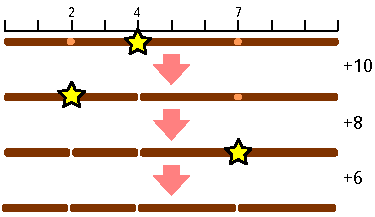
\includegraphics[width=10cm]{asset/cutting-stick-3.pdf}
\end{figure}
\end{frame}

\begin{frame}
\frametitle{Contoh Soal 2: Memotong Kayu (Solusi)}
\begin{itemize}
  \item Apakah strategi \fGreedy dengan memotong "setengah-tengahnya" selalu menghasilkan solusi optimal?
  \item Bagaimana dengan kasus jika $M = 2000$ dan $L = [1, 2, 3, 4, 5, 1000]$?
  \item Kita akan coba menggunakan DP untuk persoalan ini.
\end{itemize}
\end{frame}

\begin{frame}
\frametitle{Contoh Soal 2: Memotong Kayu (Solusi)}
\begin{itemize}
  \item Untuk pemotongan pertama, terdapat $N$ pilihan lokasi pemotongan.
  \item Jika kita memotong di posisi $L_x$, maka didapatkan dua batang.
  \item Batang pertama perlu dipotong di titik $L_1, L_2, ..., L_{x-1}$ dan batang kedua di $L_{x+1}, L_{x+2}, ..., L_N$.
  \item Ternyata kita mendapatkan sub-persoalan yang serupa.
  \item Pemotongan bisa dilanjutkan secara rekursif, dan kita pilih posisi pemotongan yang ke depannya membutuhkan usaha terkecil.
\end{itemize}
\end{frame}

\begin{frame}
\frametitle{Contoh Soal 2: Memotong Kayu (Solusi)}
\begin{itemize}
  \item Definisikan sebuah fungsi $g(x,y)$ sebagai jumlah usaha minimum yang mungkin diperoleh, jika kita hanya perlu memotong di $L_{x}, L_{x+1}, ..., L_{y}$.
  \item Untuk menghitung $g(x,y)$ kita dapat mencoba titik mana yang kita potong pertama kali.
  \item Jika kita memotong di $L_k$ $(x \leq k \leq y)$, maka kita akan mendapatkan dua potongan.
\end{itemize}
\begin{figure}
  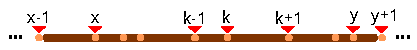
\includegraphics[width=10cm]{asset/cutting-stick-4.pdf}
\end{figure}
\end{frame}

\begin{frame}
\frametitle{Contoh Soal 2: Memotong Kayu (Solusi)}
\begin{figure}
  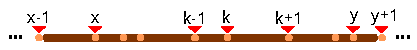
\includegraphics[width=10cm]{asset/cutting-stick-4.pdf}
\end{figure}
\begin{itemize}
  \item Total usaha yang dibutuhkan jika kita melakukan pemotongan di $L_k$ adalah jumlah dari:
  \begin{itemize}
    \item Total usaha minimum dari potongan pertama, yaitu $g(x,k-1)$.
    \item Total usaha minimum dari potongan kedua, yaitu $g(k+1,y)$.
    \item Usaha untuk pemotongan ini, yaitu $L_{y+1} - L_{x-1}$.
  \end{itemize}
  \item Untuk mempermudah, asumsikan $L_0 = 0$ dan $L_{N+1} = M$.
\end{itemize}
\end{frame}

\begin{frame} 
\frametitle{Contoh Soal 2: Memotong Kayu (Solusi (lanj.))}
\begin{itemize}
  \item Ketika $x>y$, artinya sudah tidak ada pemotongan yang perlu dilakukan.
  \item Dengan demikian, usaha yang dibutuhkan adalah 0, atau $g(x,y) = 0$.
\end{itemize}
\end{frame}

\begin{frame} 
\frametitle{Contoh Soal 2: Memotong Kayu (Solusi (lanj.))}
Dapat dirumuskan:
\begin{small}
\[g(x,y) = \left\{\begin{array}{lr}
    0, & x>y\\
    \min_{x \leq k \leq y} g(x,k-1) + g(k+1,y) + (L_{y+1} - L_{x-1}), & x \leq y \\
    \end{array}\right.\]
\end{small}
\end{frame}

\begin{frame} 
\frametitle{Contoh Soal 2: Memotong Kayu (Solusi (lanj.))}
\begin{itemize}
  \item Terdapat $O(N)$ nilai berbeda untuk nilai $x$ dan $O(N)$ nilai berbeda untuk nilai $y$ pada $g(x,y)$.
  \item Dibutuhkan iterasi sebanyak $O(N)$ untuk menghitung $g(x,y)$. 
  \item Sehingga untuk menghitung seluruh nilai $g(x,y)$ untuk seluruh $x$ dan $y$ dibutuhkan waktu $O(N^3)$.
\end{itemize}
\end{frame}

\begin{frame}
\frametitle{Contoh Soal 1: Knapsack (Pseudocode)}
Kita implementasikan $g(x, y)$ sebagai fungsi $\proc{solve}(x,y)$:
\begin{small}
\begin{codebox}
\Procname{$\proc{solve}(x, y)$}
\li \If $(x > y)$ \Then
\li   \Return $0$
\li \ElseIf $hasComputed[x][y]$ \Then
\li   \Return $memo[x][y]$ 
\li \Else
\li   $best \gets \infty$
\li   $cost \gets L[y+1] - L[x-1]$
\li   \For $k \gets x$ \To $y$ \Do
\li     $best \gets \min(best, \proc{solve}(x,k-1) + \proc{solve}(k+1, y) + cost)$
      \End  
\li   $hasComputed[x][y] \gets true$
\li   $memo[x][y] \gets best$
\li   \Return $best$
    \End
\end{codebox}
\end{small}
Jawaban ada pada $\proc{solve}(1, N)$
\end{frame}

\begin{frame}
\frametitle{Contoh Soal 1: Knapsack (Pseudocode)}
\begin{small}
\begin{codebox}
\Procname{$\proc{solve}()$}
\li \Comment Inisialisasi base case
\li \For $x \gets 0$ \To $N+1$ \Do
\li   \For $y \gets 0$ \To $x-1$ \Do
\li     $g[x][y] \gets 0$
      \End
    \End
\zi
\li \Comment Isi "tabel" mulai dari kasus yang kecil
\li \For $gap \gets 0$ \To $N$ \Do
\li   \For $x \gets 1$ \To $N-gap$ \Do
\li     $y \gets x + gap$
\li     $best \gets \infty$
\li     $cost \gets L[y+1] - L[x-1]$
\li     \For $k \gets x$ \To $y$ \Do
\li       $best \gets \min(best, g[x][k-1] + g[k+1][y] + cost)$
        \End  
\li     $g[x][y] \gets best$
      \End
    \End
\zi
\li \Return $g[1][N]$
\end{codebox}
\end{small}
\end{frame}

\begin{frame}
\frametitle{Penutup}
\begin{itemize}
  \item Perhatikan bahwa pada metode \fbottomup, pengisian "tabel" dilakukan secara "tidak biasa".
  \item Kita perlu mengisi mulai dari:
  \begin{itemize}
    \item $g[1][1], g[2][2], ..., g[N][N]$,
    \item lalu $g[1][2], g[2][3], ..., g[N-1][N]$,
    \item lalu $g[1][3], g[2][4], ..., g[N-2][N]$,
    \item lalu $g[1][4], g[2][5], ..., g[N-3][N]$,    
    \item dan seterusnya sampai $g[1][N]$.
  \end{itemize}
  \item Ingat bahwa pengisian "tabel" harus dilakukan dari kasus yang kecil ke besar.
  \item Definisi "kasus kecil" pada masalah ini adalah kayu dengan titik-titik pemotongan yang lebih sedikit.
\end{itemize}
\end{frame}

\begin{frame}
\frametitle{Penutup}
\begin{itemize}
  \item Perhatikan bahwa pada metode \fbottomup, pengisian "tabel" dilakukan secara "tidak biasa".
  \item Kita perlu mengisi mulai dari:
  \begin{itemize}
    \item $g[1][1], g[2][2], ..., g[N][N]$,
    \item lalu $g[1][2], g[2][3], ..., g[N-1][N]$,
    \item lalu $g[1][3], g[2][4], ..., g[N-2][N]$,
    \item lalu $g[1][4], g[2][5], ..., g[N-3][N]$,    
    \item dan seterusnya sampai $g[1][N]$.
  \end{itemize}
  \item Ingat bahwa pengisian "tabel" harus dilakukan dari kasus yang kecil ke besar.
  \item Definisi "kasus kecil" pada masalah ini adalah kayu dengan titik-titik pemotongan yang lebih sedikit.
\end{itemize}
\end{frame}

\begin{frame}
\frametitle{Penutup}
\begin{itemize}
  \item Dari contoh ini kita mempelajari bahwa urutan pengisian "tabel" pada DP \fbottomup tidak selalu biasa.
  \item Jika urutan pengisiannya salah, maka hasil akhir yang didapatkan juga bisa jadi salah.
  \item Hal in terjadi ketika kita hendak menyelesaikan kasus yang besar, tetapi hasil untuk kasus-kasus yang lebih kecil belum tersedia.
  \item Untuk mengetahui urutan pengisian "tabel", Anda perlu mengamati apa definisi "kasus kecil" pada masalah yang dihadapi.
\end{itemize}
\end{frame}

\begin{frame}
\frametitle{Ringkasan}
\begin{itemize}
  \item Terdapat dua versi DP, yaitu \ftopdown dan \fbottomup.
  \item Keduanya memiliki keuntungan dan kerugian, pilih yang tepat sesuai dengan kebutuhan soal.
  \item Kunci dari mengerjakan soal DP adalah mengidentifikasi pilihan keputusan yang bisa diambil, dan merumuskannya menjadi rumus rekursif.
\end{itemize}
\end{frame}

\begin{frame}
\frametitle{Penutup}
\begin{itemize}
  \item DP merupakan topik yang cukup luas untuk dibicarakan.
  \item Banyak berlatih mengerjakan soal DP dapat melatih kita untuk mendapatkan rumus DP yang sesuai dengan masalah yang dihadapi.
  \item Topik optimisasi lainnya pada DP akan dibahas pada kesempatan yang lain.  
\end{itemize}
\end{frame}

\end{document}
